\section{DSMC algorithm}
The current implementation of the DSMC model does a fine job simulation dilute gases in arbitrary geometries, but there is always room for improvements. The code can be optimized even more so that it runs more efficiently or requires less memory. The simulator can incorporate other physical models into the same program, increasing the useability even further. In this section we discuss some ideas that could be implemented, both from a physical point of view, and a computer science point of view.
\subsection{Sparse voxel octree}
As discussed in section \ref{sec:dsmc_binary_representation}, we have chosen a three-dimensional grid of voxels to representate the geometry. The required amount of memory for an $N\times N\times N$ grid scales as $N^3$ which rather quickly becomes a limitation. Each voxel contains one unsigned char representing the value of that voxel, in addition to nine floats being the two tangent vectors and the normal vector. This means that each voxel requires 40 bytes of memory and disk space. A geometry on a $1024\times1024\times1024$ grid then requires 43 gigabytes of memory, and since each processor has a copy of the voxels on its 26 neighbors, we then a total of 1.160 terabytes of memory. Since the grid matrix mostly consists of either zeros (for a high porosity system) or ones (for a low porosity system), we can represent the grid as a sparse voxel octree\cite{laine2011efficient}. An octree is a geometrical data structure where each volume element (a cubic box), or node, is divided into its eight equally sized children which again are divided into their eight (smaller) children.  This is repeated recursively until we have the desired grid resolution, see figure \ref{fig:future_work_octree}. 
\todo{Cite wikipedia octree page}
\begin{figure}[h]
\begin{center}
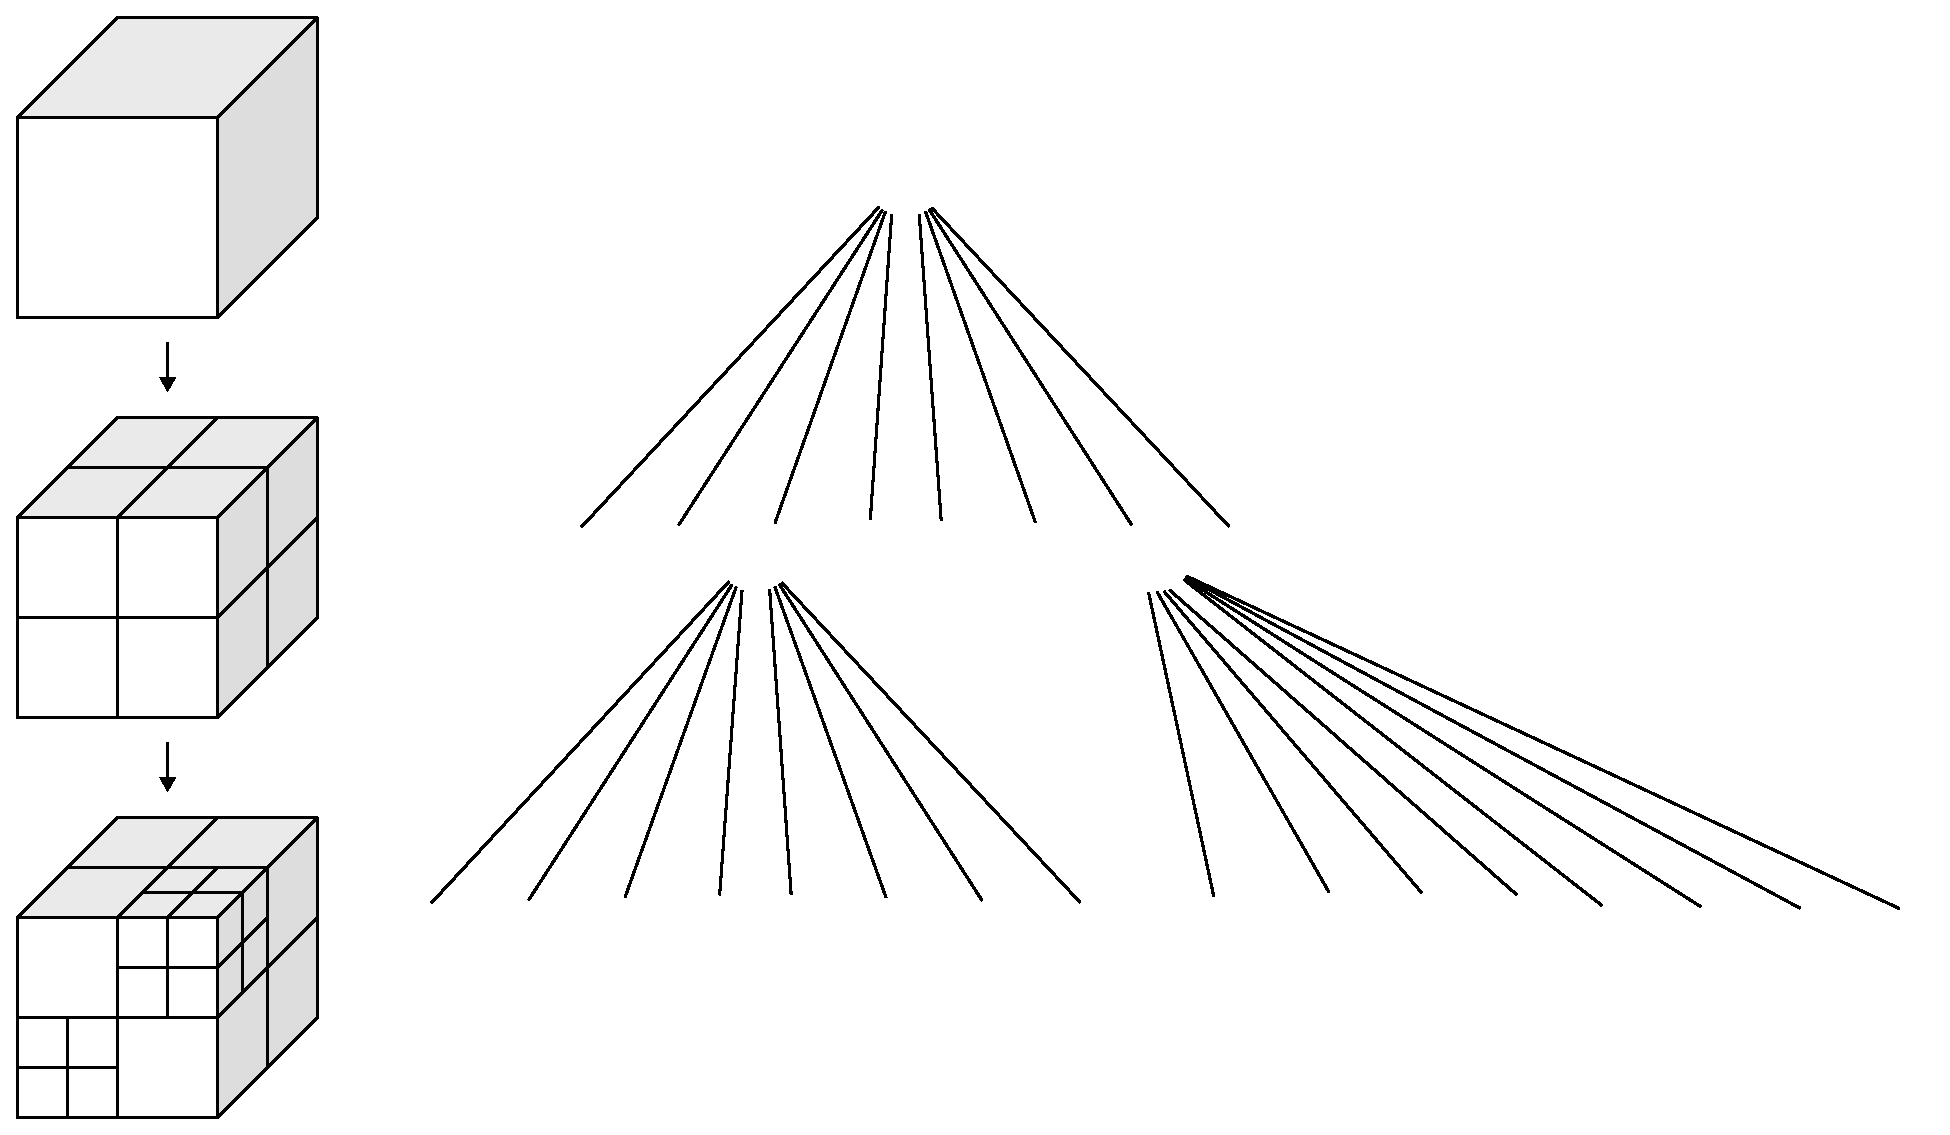
\includegraphics[width=\textwidth, trim=0cm 0cm 0cm 0cm, clip]{figures/octree.eps}
\end{center}
\caption{stuff}
\label{fig:future_work_octree}
\end{figure}
The octree is just the three-dimensional version of a binary tree. If all eight children of a node have the same value, instead of saving all the children (plus their children and so on), we just mark that node with the specific value. Doing this can save enormous amounts of memory allowing us to use a high resolution grid (which can be desired for very detailed, complex geometries).

\subsection{Load balancing}
\label{sec:future_work_load_balancing}
The parallelization technique we have used in this thesis distributes the total physical volume equally to all processors so that they compute on gas in equal volumes. Since we study porous media, parts of the total volume are a solid, not available for the gas particles. This can lead to huge deviations in the work load for each processor. A worst case scenario would appear when a processor has zero volume available for particles. In this situation, the processor does not contribute to the simulation since it has no particles. It will finish its timestep very quickly just waiting for the other processor to finish their timesteps. In the DSMC program, this will show up as large MPI Communication times (this happens because the processor reaches the MPI synchronization). In figure \ref{dsmc:mpi_waiting_time_load_balancing}, we have plotted the MPI Communitation time distribution across 512 processors for a system \todo{Describe the system}. A solution to this would be to adjust the size of the volumes each processor controls so that the number of particles per processor is approximately equal. 
\missingfigure{MPI Waiting time distribution}
\subsection{Large system state preparation}
When studying flow, we need the system to reach a steady state before we can start measuring statistical properties of the system. This process can take quite a while 
\subsection{Diffusion on the matrix}

\subsection{Deformations and fracking}
\section{MD algorithms}

\section{Multi scale physics}
\subsection{From MD to DSMC}
\section{Excellent physical questions}
\subsection{Vanishing statistical spread for large systems}
\subsection{Permeability of real materials}